\begin{frame}
    \frametitle{LED}
    \begin{center}
        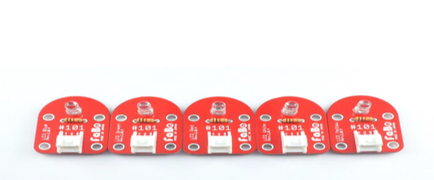
\includegraphics[width=0.8\textwidth]{images/chap05/text05-img016.png}
        \begin{itemize}
            \item 値が1のとき光る
            \item 値が0のとき消える
        \end{itemize}
    \end{center}
    \textpageref{9}
\end{frame}

\begin{frame}
    \frametitle{\makebox[50pt][l]{\ruby{振動子}{しん|どう|し}}}
    \begin{center}
        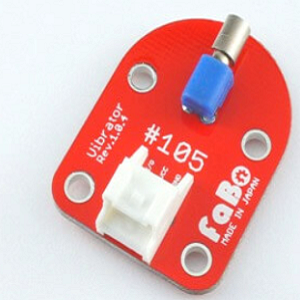
\includegraphics[width=0.4\textwidth]{images/chap05/text05-img017.png}
        \begin{itemize}
            \item 値が1のとき\ruby{震}{ふる}える
            \item 値が0のとき動かない
        \end{itemize}
    \end{center}
    \textpageref{9}
\end{frame}

\begin{frame}
    \frametitle{センサーをピンにつけてみよう}
    \begin{center}
        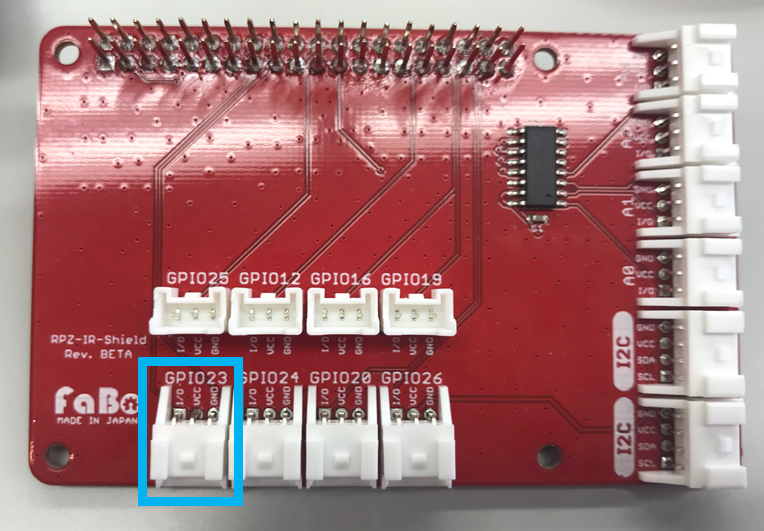
\includegraphics[width=0.4\textwidth]{images/chap05/text05-img027.png}
        \begin{itemize}
            \item GPIO23とLEDをつなげてみよう
            \item HSPで	\textasciitilde/05/digout.hsp を動かしてみよう
        \end{itemize}
    \end{center}
    \textpageref{12}
\end{frame}

\begin{frame}[fragile]
    \frametitle{デジタル出力センサを使った\\プログラム}
    \begin{lstlisting}[title=\textasciitilde/05/digout.hsp]
    #include "hsp3dish.as"
    #include "rpz-gpio.as"

    *main
        redraw 0
        font "",20
        pos 20,20
        mes "センサーが動いたり止まったりします"
        redraw 1

        gpio 23,1
        wait 100
        gpio 23,0
        wait 100
        goto *main
    \end{lstlisting}
    \textpageref{12}
\end{frame}

\begin{frame}[fragile]
    \begin{exampleblock}{問題を解いてみよう}
        \begin{itemize}
            \item 教科書13ページ 問題5-4(2問)
        \end{itemize}
    \end{exampleblock}
\end{frame}